
For this event type, full-scale floor loads are generated utilizing wind tunnel data made available by Tokyo Polytechnic University, specifically their \href{http://wind.arch.t-kougei.ac.jp/system/eng/contents/code/tpu}{TPU Aerodynamic Database}. The TPU Aerodynamic database provdes a number of databases. Currently this tool utized data provided for \href{http://www.wind.arch.t-kougei.ac.jp/info_center/windpressure/lowrise/mainpage.html},{Low Rise Buildings Without Eaves}. That database provides wind tunnel data of wind-loads on low-rise buildings: gable, hip, and flat roofed buildings. Information on the data and how it was obtained is provided in their \href{http://www.wind.arch.t-kougei.ac.jp/info_center/windpressure/lowrise/Introductionofthedatabase.pdf} documentation. The imporatnt wind field information: The turbulence density at a height of 10cm was about 0.25.  The test mean wind velocity at this height was about 7.4m/s, corresponding to about 22m/s at a height of 10m in full scale. The tests were performed on a limited number of buildings with different aspect ratios and wind coming from different angles on the building.

As wil be discussed in the theory section, the wind loads are obtained from the pressure tap data by determining a length factor and a velocity factor. The length factor is determined from the building height. The forces, unlike in DEDM-HRP, are determined given the building dimensions provided in the general information sheet and the length and velocity factors.

\begin{figure}[!htbp]
  \centering {
    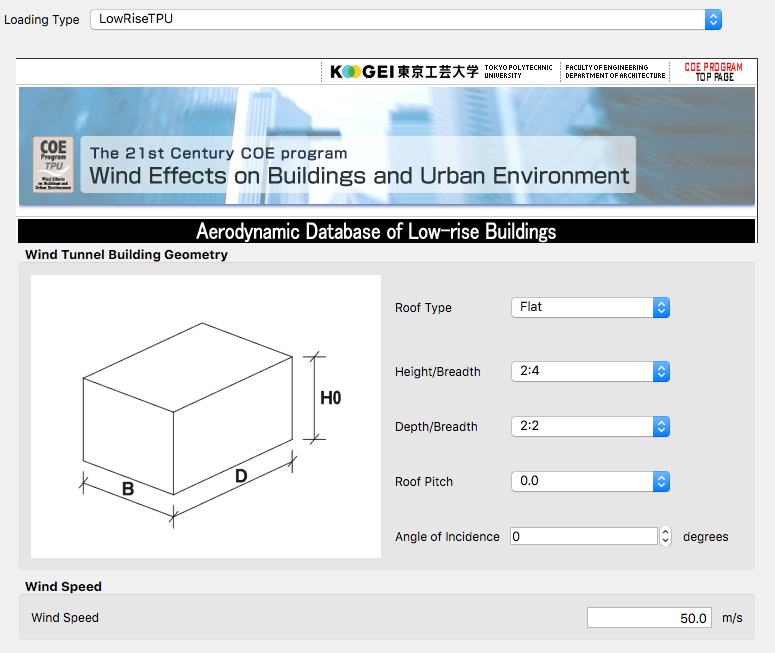
\includegraphics[width=0.8\textwidth]
    {usage/figures/lowRiseTPU.png} }
  \caption{Low Rise TPU Wind Loading Event}
  \label{fig:lowRiseTPU}
\end{figure}

In the inputs for the event, as shown in figure \Cref{fig:lowRiseTPU} require the user to specify which 
of these tests to use:
\begin{enumerate} 
\item The roof type, currently only flat is an option.
\item The user specifies one of 4 height to breadth ratios.
\item One of three depth to breadth ratios.
\item A roof picth.
\item The angle of incidence, 0 through 90 in 15 degree increments.
\item Mean Wind Speed: The wind speed provided is used in determing the velocity factor and the applied loads. 
\end{enumerate}

Random Variables: For this event, the wind speed can be a random variable.

